\documentclass[12pt]{extarticle}
% Some packages I commonly use.
\usepackage[english]{babel} \usepackage{graphicx} \usepackage{framed}
\usepackage[normalem]{ulem} \usepackage{amsmath} \usepackage{amsthm}
\usepackage{amssymb} \usepackage{multirow} \usepackage{multicol}
\usepackage{adjustbox} \usepackage{amsfonts} \usepackage{enumerate}
\usepackage[utf8]{inputenc} \usepackage[top=1 in,bottom=1in, left=1 in, right=1
in]{geometry} \usepackage{hyperref} \usepackage{xcolor} \usepackage{rotating}
\usepackage{booktabs} \usepackage{subfig} \usepackage[strict]{chngpage}
\usepackage{textcomp}
% \usepackage{subcaption} \usepackage[sc]{caption}
\usepackage{float} \usepackage{soul} % testo barrato
\usepackage{enumitem}

% A bunch of definitions that make my life easier
\newlist{SubItemList}{itemize}{1} \setlist[SubItemList]{label={$-$}}

\let\OldItem\item \newcommand{\SubItemStart}[1]{%
  \let\item\SubItemEnd
  \begin{SubItemList}[resume]%
    \OldItem #1%
  } \newcommand{\SubItemMiddle}[1]{%
    \OldItem #1%
  } \newcommand{\SubItemEnd}[1]{%
  \end{SubItemList}%
  \let\item\OldItem
\item #1%
} \newcommand*{\SubItem}[1]{%
  \let\SubItem\SubItemMiddle%
  \SubItemStart{#1}%
}%

\newcommand{\matlab}{{\sc Matlab} } \newcommand{\cvec}[1]{{\mathbf #1}}
\newcommand{\rvec}[1]{\vec{\mathbf #1}} \newcommand{\ihat}{\hat{\textbf{\i}}}
\newcommand{\jhat}{\hat{\textbf{\j}}} \newcommand{\khat}{\hat{\textbf{k}}}
\newcommand{\minor}{{\rm minor}} \newcommand{\trace}{{\rm trace}}
\newcommand{\spn}{{\rm Span}} \newcommand{\rem}{{\rm rem}}
\newcommand{\ran}{{\rm range}} \newcommand{\range}{{\rm range}}
\newcommand{\mdiv}{{\rm div}} \newcommand{\proj}{{\rm proj}}
\newcommand{\R}{\mathbb{R}} \newcommand{\N}{\mathbb{N}}
\newcommand{\Q}{\mathbb{Q}} \newcommand{\Z}{\mathbb{Z}} \newcommand{\<}{\langle}
\renewcommand{\>}{\rangle} \renewcommand{\emptyset}{\varnothing}
\newcommand{\attn}[1]{\textbf{#1}} \theoremstyle{definition}
\newtheorem{theorem}{Theorem} \newtheorem{corollary}{Corollary}
\newtheorem*{definition}{Definition} \newtheorem*{example}{Example}
\newtheorem*{note}{Note} \newtheorem{exercise}{Exercise}
\newcommand{\bproof}{\bigskip {\bf Proof. }}
\newcommand{\eproof}{\hfill\qedsymbol} \newcommand{\Disp}{\displaystyle}
\newcommand{\qe}{\hfill\(\bigtriangledown\)} \setlength{\columnseprule}{1 pt}
\newcommand*\rfrac[2]{{}^{#1}\!/_{#2}}

\begin{document}

\begin{figure}[]
  \centering {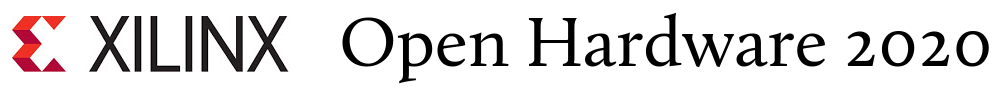
\includegraphics[width=1.0\textwidth]{images/xilinxoh.png}}
\end{figure}

\begin{figure}[]
  \centering \vspace{1cm}
  {
\includegraphics[width=.15\textwidth]{images/Padova.png}}
\end{figure}
% \vspace{-0.5cm}
\begin{center}
  {\large{U}\normalsize{NIVERSITÀ DEGLI}\large{ S}\normalsize{TUDI DI}\large{ P}\normalsize{ADOVA}}\\
  % \textit{Corso di Dottorato in Physics}\\
  % {\small{Anno accademico 2018-2019}}\\
  \textit{ }\\
  \textit{ }\\
  \textit{ }\\
  \textit{ }\\
  \textbf{\large{Documents Submission for Xilinx Open Hardware 2020}}\\
  \textit{ }\\
  \textit{ }\\
  \textit{ }\\
  \textit{\Large{Report on the 'NCO based CDR implementation in FPGA'}} \\
  \textit{ }\\
  \noindent\rule{16cm}{0.4pt}
  \textit{ }\\
  \textit{ }\\
  \textit{ }\\
  \textbf{Team number: xohw20\_203}\\
  \textit{ }\\
  Team Partecipant: Filippo Marini$^1$\\
  \textit{ }\\
  Team Supervisor: Dr. Ing. Marco Bellato$^2$\\
  \textit{ }\\
\end{center}

\textit{ }\\
$1$: Universita' degli Studi di Padova, INFN Padova. \textit{filippo.marini@pd.infn.it}\\
$2$: INFN Padova. \textit{marco.bellato@pd.infn.it}\\
\newpage

\section{Introduction}
The capability to extract timing informations out of a serial data stream to
decode the incoming informations has become a very common requirement. To sample
the incoming data, the receiver usually relies on a Clock and Data Recovery
(CDR) chip, which generates a clock signal at the corresponding sampling
frequency, phase-aligned to the data. Modern physics experiment have often this
same requirement, where perhaps thousands of boards receive uncorrelated data
and it's up to them to decode the messages. For that reason, the presence of a
CDR on-board is usually mandatory. Present readout systems in physics
experiments usually rely on FPGAs to receive and transmit data at high rate to
high capaicity DAQ systems; exploting FPGAs to recover timing information from
streamed data is therefore beneficial for a number of reasons, including power
consumption and cost reduction. \\
The design is based on two components: a Numerically-Controlled Oscillator
(NCO), in order to create a controlled frequency clock signal, and a digital
Phase Detector (PD) to match the clock frequency with the data rate. NCOs are
often coupled with a Digital to Analog Converter (DAC) to create Direct Digital
Synthesizers (DDS), which are able to produce analog waveforms of any desired
frequency. In the presented case, the NCO generates a digital clock signal of an
arbitrary frequence, while the PD manages this frequency by intercepting any
shifting on the relative phase between the clock and the data.

\subsection{Possible Application}
The design finds a possible application in the context of the Jiangmen Neutrino
Observatory [note!!] (JUNO), a 20 kton liquid scintillator detector neutrino
physics experiment where the charge information of the incident neutrinos will
be retrieved by 18'000 20-inches PhotoMultipliers Tubes (PMT) surrounding the
central detector. The proposed CDR would be part of the timing and trigger
system of the Front-End/Back-End electronics, which
features a custom synchronous link protocol.\\
JUNO employs this link with a star topology, where the hub, consisting of a
Back-End Card (BEC), connects to 48 Front-End card, the so-called Global Control
Unit (GCU). The physical link consists
of a standard CAT5e Foil Twisted Pair (FTP) cable, up to about 100 meters long.\\
The four twisted pairs transport
\begin{itemize}
\item 125 Mbps Trigger requests (GCU to BEC)
\item 125 Mbps Synchronous messages (Bidirectional)
\item 62.5 MHz Digital Clock (BEC to GCU)
\end{itemize}
To get rid of the AC imbalance, the synchronous messages are Manchester encoded
(plus Hamming encoded for 1 bit error correction), while the trigger requests
use a scrambler mechanism, to avoid any bandwidth waste. While the BEC features
an automatic channel calibration that ensures
the correct decoding of the data, the GCU needs to rely on a CDR mechanism.\\
The proposed CDR project would be a perfect fit.

\section{Specifications}
The CDR core provides the High Range (HR) pins of the Xilinx Kintex-7 FPGA with
clock and data recovery capability. The use of HR general purpose I/O pins over
dedicated transceivers is allowed by the relatively low expected data-rates (up
to 250 Mbps), granting the project with reduced power consumption and a more
straightforward design. Moreover, the core is easily portable to a different
Xilinx FPGA family which features dynamic-phase-controlled clock management
tiles and a SerDes I/O tile. \bigbreak Some of the specifications are:
\begin{itemize}
\item Clock and Data recovery tested from 62.5Mbps up to 250Mbps NRZ data
  stream.
\item Controllable phase relationship between recovered clock and data streaming
\item Dynamic CDR locked flag
\item Latency for CDR locking to data: several seconds
\item Selectable reference frequencies
\item Clock and data recovery capability not affected after 100 meters of CAT5e
  cable
\item Input ports:
  \begin{itemize}
  \item System clock: board system clock (\textit{i.e.}, Clock from on-board
    crystal)
  \item incoming data streaming to decode
  \item Input from recovered clock external loopback (see Sec. ??)
  \end{itemize}
\item Ouput ports:
  \begin{itemize}
  \item Output for recovered clock external loopback (see Sec. ??)
  \item Recovered clock
  \end{itemize}
\item Debug interface ports and generics:
  \begin{itemize}
  \item Frequency change requests report (forwarded to the NCO from the phase
    and frequency detector)
  \item Possibility to use Xilinx VIO to set recovered clock frequency
  \item several LED reporting the locking status of MMCMs, CDR locking status
    and presence of data stream.
  \end{itemize}
\end{itemize}

\section{Architecture}
\subsection{Overview}
The block diagram of the core is given in Figure~\ref{fig:cdr_overview}.

\begin{figure}[H]
  \centerline{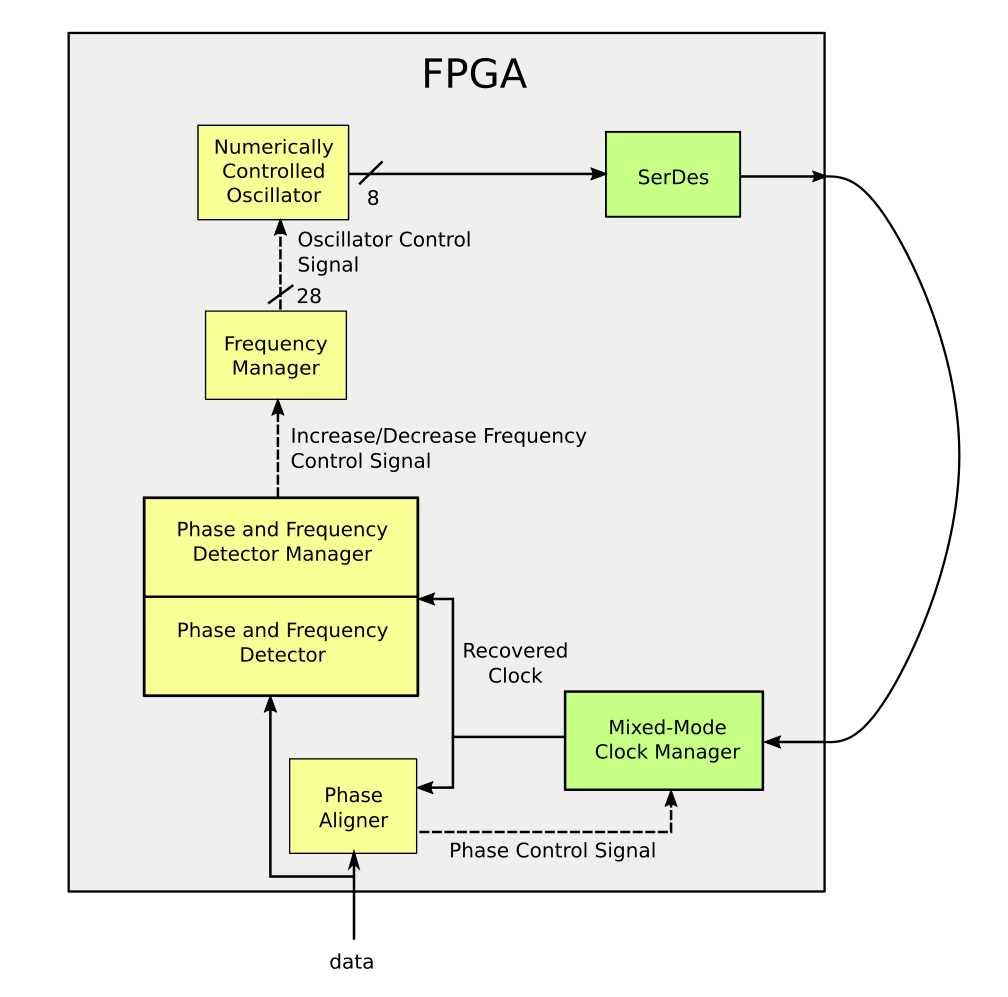
\includegraphics[width=0.5\linewidth]{images/block}}
  \caption{Block diagram for the proposed CDR design. Yellow blocks represents
    custom VHDL modules, green blocks are used to represent FPGA proprietary
    tiles. Dashed lines are used for control signals.}
  \label{fig:cdr_overview}
\end{figure}

The CDR mechanism is similar to the usual PLL architecture, where the phase of a
reference signal is compared to the phase of an adjustable feedback signal,
generally provided by a controlled oscillator, like a Voltage Controlled
Oscillator (VCO). When the phase comparison is in steady state, e.g. the phase
and frequency of the reference signal is equal to the phase and frequency of the
feedback signal, we say that the PLL is locked. In the case of a CDR, the steady
state is reached when the VCO clock frequency
matches the reference signal's data rate.\\
The PLL's VCO is substitued in the core's design by a Numerically Controlled
Oscillator (NCO) which is used to create a frequency controlled clock. The
frequency comparator's job is carried out by a Phase and Frequency Detector
(PFD) monitoring the NCO's clock frequency to match it with the data rate, and a
Phase Aligner (PA) that, together with the Xilinx 7 Series MMCME2\_ADV tile
[cite!!], dynamically adjusts residual clock drifting and have a deterministic
phase
relationship with the incoming data stream.\\

\subsection{Numerically Controlled Oscillator}
To generate a controlled frequency clock signal, an NCO is employed by the core.
Its design consist of two parts:
\begin{itemize}
\item A Phase Accumulator (PACC), which is basically a counter incremented by a
  reference clock.
\item A phase-to-amplitude converter, which uses the PACC output as an index to
  a pseudo-Look-Up Table (LUT)
\end{itemize}
To understand the NCO operation, we can think of a vector rotating around a
phase-circle (Figure ??). To each point of this phase-wheel corresponds a
defined value. One revolution of the vector around the phase-wheel, at costant
speed, results in one complete cycle of the output wave. The PACC counter value
corresponds to the points around the phase-wheel, while the pseudo-LUT assign a
specific value to each point. The PACC output value is increased every system
clock cycle, by a specific amount, the \textit{jump size} (\textit{M} in the
picture). The jump size, together with the number of points
in the wheel, defines the output wave's frequency.\\
The correlation between the jump size, the reference clock and the output
waveform frequency is
\begin{equation}
  f_{OUT} = \frac{M \times f_C}{2^N}
  \label{eq:f_out}
\end{equation}
where:
\begin{itemize}
\item $M$ is the jump size
\item $f_{OUT}$ is is the NCO output waveform frequency
\item $f_C$ is the reference clock frequency
\item $N$ is the number of bits dedicated to the PACC counter
\end{itemize}
In order to create a square wave clock signal, the pseudo-LUT assign to half of
the circle the value of '1' while on the other half the value of '0'. This is
done just by taking a specific bit of the PACC counter (hence why the LUT has
been called 'pseudo').\\
However, this desig presents a limitation on the phase resolution: since the
output signal is digital, the time domain is discrete and it corresponds to the
system clock period. This implies the the positive (and negative) fraction of
the output clock signal can only be a multiple of this time domain resolution,
making the output frequency only \underline{on average} determined by the jump
size of the accumulator. Also, the maximum obtainable output clock frequency
employing this architecture is half of the system clock, which makes it hard to
reach a frequency of 250 MHz, needed for data rates of 250 Mbps.\\
In the next chapter, a way to increase the phase resolution is illustrated. This
will allow the design to work with data rates up to 250 Mbps.\\

\subsubsection{The SerDes Technique}
As a first approach, to improve the phase resolution as well as the output clock
frequency, the system clock shall be increased. This decreases the system clock
period (which equals to the NCO clock phase resolution) and increases the $f_C$
value on Eq.~\ref{eq:f_out}.\\
Even though this approach actually helps to resolve the issues, the reference
clock frequency must comply with the FPGA architecture and can not be increased
over a certain threshold to avoid timing errors.\\
A different approach consist in exploiting the parallelism capability of the
FPGA: instead of just creating one phase-wheel, we generate several of them,
with equal number of points and equal jump size. However, the rotating vector of
these phase-wheels will not compute the same points of the wheel, but they will
span the gap between the phase-points landed by the vector of the first
phase-wheel. After the pseudo-LUT will give value to the phase-points of the
different
wheels, the results are serialized by a SerDes.\\
To clarify, fig. ?? presents an example where two phase-wheels are being
generated. For graphical reason, the output will be
represented as a sine waveform instead of a digital 50\% duty cycle clock.\\
The reference clock has a frequency of 250 MHz, therefore every phase-wheel
evaluates a phase-point every 4 ns (Note that the green and blue points are
computed at the same time) and applying eq.~\ref{eq:f_out}, the resulted
waveform's frequency is 62.5 MHz.\\
To compute the offset in phase-points between each wheel, we refer to the
following equation:
\begin{equation}
  \text{\textit{offset}} = \frac{M}{PW}
  \label{eq:offset}
\end{equation}
where $PW$ is the number of phase-wheels generated and $M$ is the jump size
(Note that $M$ must be equal or greater than $PW$. If the result is fractional,
$\text{\textit{offset}}$ is approximated to the closest integer).\\
By employing 8 phase-wheels in the CDR core's design with a system clock of 250
MHz, the phase resolution goes from 4 ns to 500 ps. The serialization of the 8
digital bits generated by the pseudo-LUT is carried out by the OSERDESE2 I/O
Kintex 7 tile. Since the OSERDESE2 output must be connected to an I/O Block
(IOB) only, a loopback in and out of the FPGA is a precondition to be foreseen
when designing the Printed Circuit
Board (PCB) hosting the FPGA.\\

\subsection{Phase and Frequency Detector}
To match the NCO clock frequency with the data rate, a \textit{Phase and
  Frequency Detector} (PFD) is employed by the core.\\
The PFD frequency detection capability relies on the use of two clock signals,
whose frequency is given by the NCO, with 50\% duty cycle and orthogonal with
each other ($\pi/2$ phase difference). The rising ad falling edges of these two
signals allos the division of the entire 360 degrees of the clock period into
four quadrants, as shown in Fig. ??. If the data edges drift up or down these 4
quadrants, the NCO frequency does not
match the data rate, and needs to be adjusted.\\
The first stage for the data-edges quadrant identification is carried out by the
\textit{Phase Detector Unit} which features a couple of Alexander-type Bang-Bang
phase detectors connected to the two orthogonal clock waves. Their outputs
consists in early/late pulses (early means that the data has its edge in the
positive half of the clock signal, late correspond to the data edge in the
negative half) which are then passed, after a filtering stage based off an
early/late counter, to the \textit{Frequency Detector Unit}. In here two
modules, the \textit{Quadrant Detector} and the \textit{Quadrant Shifting
  Detector} are able to
\begin{itemize}
\item First, detect the current quadrant where the data edges resides, based on
  the early/late information coming from the two phase detectors of the
  \textit{Phase Detector Unit}
\item Second, store and analyze this information in order to monitor the
  shifting of the data edges quadrant and dictate whether the clock frequency is
  faster or slower than the data rate.
\end{itemize}
When the decision is taken, a \textit{shifting} flag is issued, reporting to the
\textit{Phase and Frequency Detector Manager} in which direction the data edges
are 'climbing' the clock quadrants. !!! Figure tutte o solo PFD?? !!!

\subsection{Phase and Frequency Detector Manager}
Since it is impossible for the clock frequency to perfectly equal the data rate,
due to the finite resolution of the clock frequency and real-world conditions
(\textit{i.e.}, jitter, setup/hold vilations ...), the \textit{Phase and
  Frequency Detector Manager} module exploits a counter method with several
different threshold to get the closest possible frequency as
well as driving the \textit{CDR locked} flag.\\
The counter is set to increase its value when the PFD reports a fester clock
compared to the data, while it decreases on the opposite case. The different
threshold with the related scenarios are:
\begin{itemize}
\item $\pm$ \textit{lock threshold} (around 10\% of the maximum value): inside
  this range the CDR is locked.
\item $\pm$ \textit{activate threshold} (around 50\%): when locked, outside this
  range a frequency change request is forwarded to the NCO.
\item $\pm$ \textit{unlock threshold} (around 90\%): if exceeded, the CDR lock
  flag gets deasserted.
\end{itemize}
Any frequency change request is passed to the \textit{Frequency Manager} module
which adjust the phase-wheel jump size accordingly.\\
When delivering the increase/decrease requests to the \textit{Frequency Manager}
module, the logic signals intersect Clock Domain Crossing (CDC) boundaries. The
PFD design unit is in the NCO's clock domain, while the \textit{Frequency
  Manager}, as well as the NCO itself, are synchronized with the
system clock.\\
To comply with the CDC boundary crossing, a control signal is sent together with
the request, to avoid erroneous sampling [cite!!]. A timing diagram is
shown in fig. ??.



\end{document}
